\documentclass[14pt]{extarticle}
\usepackage[english,ukrainian]{babel}
\usepackage[utf8]{inputenc}
\usepackage{amsmath,amssymb}
\usepackage{parskip}
\usepackage{graphicx}
\usepackage{tcolorbox}
\tcbuselibrary{skins}
\usepackage[framemethod=tikz]{mdframed}
\usepackage{chngcntr}
\usepackage{enumitem}
\usepackage{float}
\usepackage{subfig}
\usepackage{esint}
\usepackage[top=2.5cm, left=3cm, right=3cm, bottom=4.0cm]{geometry}
\usepackage[table]{xcolor}
\usepackage{algorithm}
\usepackage{algpseudocode}
\usepackage{listings}
\usepackage{dsfont}

% Chad's colors:
% See http://web.njit.edu/~kevin/rgb.txt.html for possibilities
\definecolor{ChadDarkBlue}{rgb}{.1,0,.2}  
\definecolor{ChadBlue}{rgb}{.1,.1,.5}  
\definecolor{ChadRoyal}{rgb}{.2,.2,.8}  
%\definecolor{ChadGreen}{rgb}{0,.35,.1}
%\definecolor{ChadGreen}{rgb}{0,.5,.25}  % Too bright
%\definecolor{ChadGreen}{rgb}{0,.4,.2}    % Still too bright
\definecolor{ChadGreen}{rgb}{0,.4,0}    % Dark Green
%\definecolor{ChadRed}{rgb}{.8,.1,.2}    % Too bright
\definecolor{ChadRed}{rgb}{.5,0,.5}  % purple

%%% HYPERLINKS %%%%%%%%%%%%%%%%%%%%%
\usepackage[colorlinks,breaklinks,   % deleted ps2pdf 11/6/15
     bookmarks=false,
     pdfstartview=Fit,  % for fitting entire page; FitW just fits width
     pdfview=Fit,       % after traversing a hyperlink
     linkcolor=ChadRed,
     urlcolor=ChadRed,
     citecolor=ChadGreen,
     hyperfootnotes=false
         ]{hyperref}
\usepackage[figure,table]{hypcap} % Correct a problem with hyperref
\urlstyle{rm} % so it doesn't use a typewriter font for url's.
\usepackage[nameinlink]{cleveref}

\title{Домашня робота \#1 з курсу ``Моделювання на \textit{Python}''}
\author{Студента 3 курсу групи МП-31 Захарова Дмитра}
\date{\today}

\begin{document}

\maketitle

\section*{Умова}

Розглядається спрощена задача \textit{перколяції}. На полі $n\times n$ кожна клітинка з ймовірністю $p$ стає ``перешкодою''. Далі у найвищий рядок (товщина 1 клітинка) ставиться рідина, котра кожен хід заповнює пусті клітинки. Питання -- з якою ймовірністю знайдеться шлях між найвищим і найнижчим рядком? Цей процес проілюстровано на рис. \ref{fig:percolation}.

\begin{figure}
    \centering
    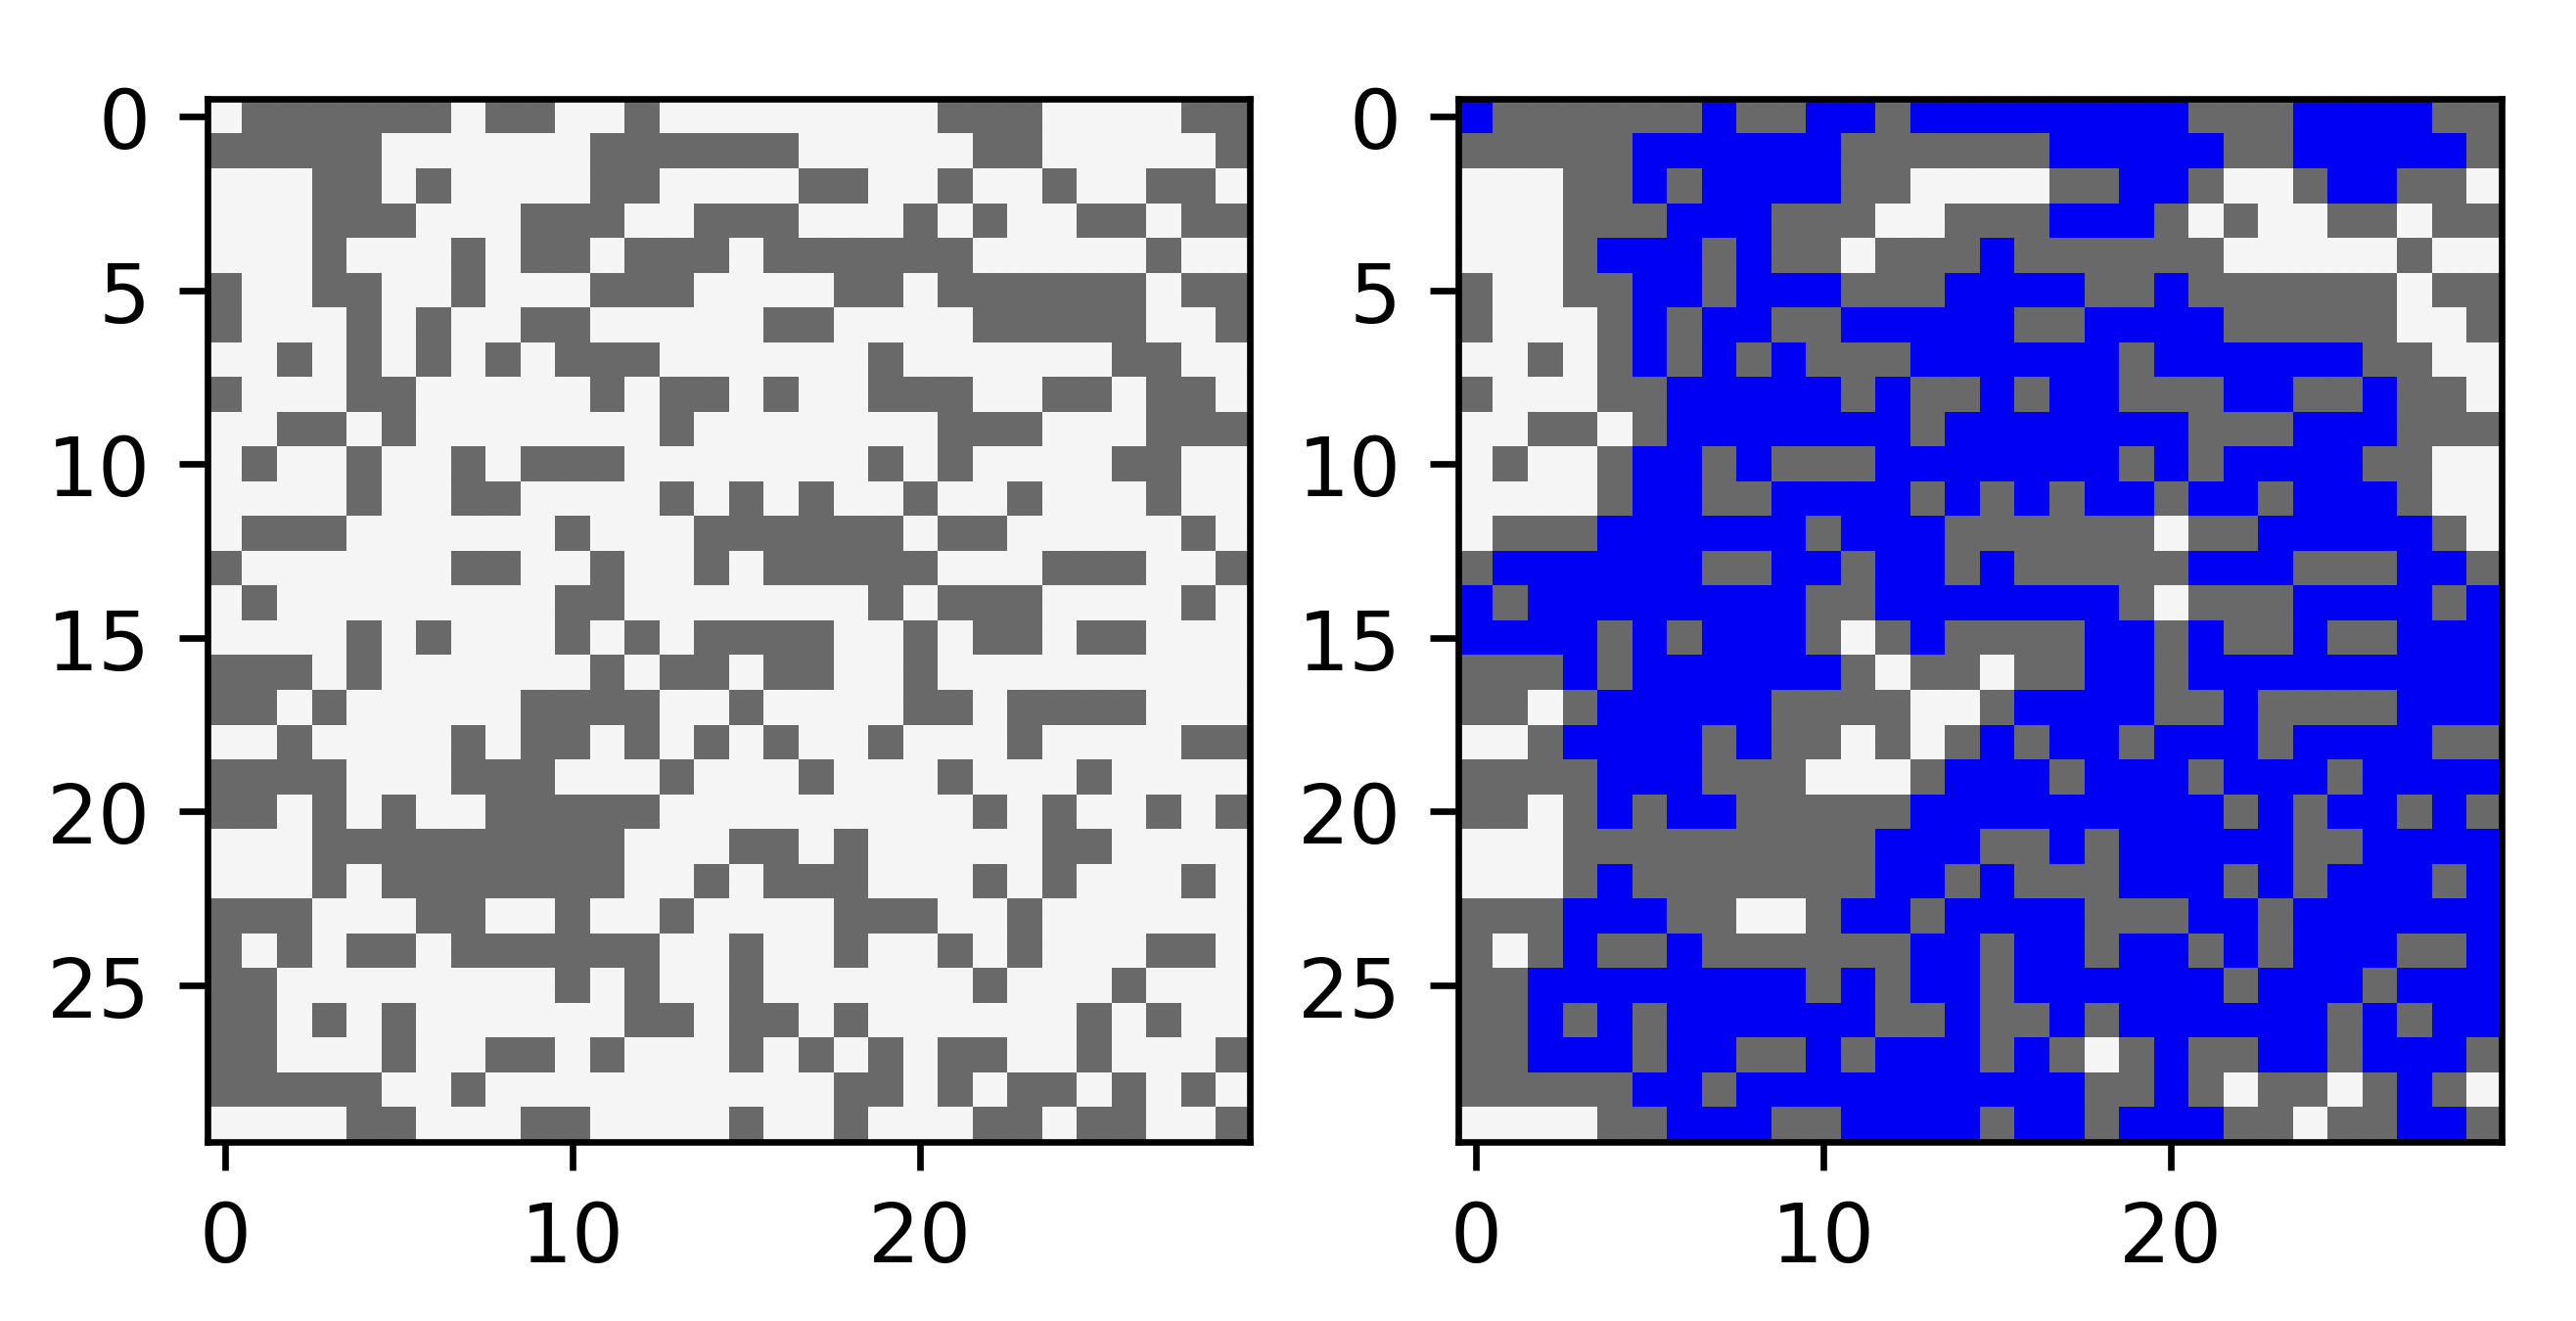
\includegraphics[width=0.53\textwidth]{images/hw_1/illustration.png}
    \caption{Процес перколяції. На рис. ліворуч показано початкову конфігурацію до додавання рідини. Праворуч -- після того, як рідина ``розтіклась'' по місцевості.}
    \label{fig:percolation}
\end{figure}

\section{Програма}

\textbf{Умова.} Спробуйте провести свої експерименти, написавши свою програму та/або змінюючи параметри задачі.

\textbf{Відповідь.} Код програми наведений за \href{https://github.com/ZamDimon/University-Homeworks/tree/main/Term%206/Modelling%20in%20Python/code/homework_1}{цим \textit{GitHub} посиланням}. Головна відмінність від наведеного у завданні -- це невеличка реорганізація коду. Тепер, у класі \texttt{TileType} можна вказувати колір клітинок, у класі \texttt{Grid} відбувається основна логіка перколяцій, а у файлі \texttt{cli.py} можна зручно викликати одну з трьох команд:
\begin{itemize}
    \item \texttt{python3 cli.py instant-fill} -- показується картинка ``до'' і ``після'' руху ``рідини'';
    \item \texttt{python3 cli.py animation-fill} -- те саме, але з анімацією;
    \item \texttt{python3 cli.py analyze-depth} -- проводиться багато експериментів при різних параметрах $p \in [p_{\min},p_{\max}]$ і рахується статистика для кожного $p$ (детально про це в секції \ref{section:problem_2}).
\end{itemize}

\section{Аналіз}\label{section:problem_2}

\textbf{Умова.} Допишіть фрагмент програми, який дозволяє дізнатися, чи відбулася перколяція. Спробуйте експериментально знайти величину $p$, для якої перколяція скоріш за все виникне. Запишіть результати своїх експериментів і зробіть висновки.

\textbf{Розв'язання.} Для аналізу ми додали функцію \texttt{\_instant\_fill}, котра робить дві речі:
\begin{enumerate}
    \item Ставить рідину у перший рядок і рахує її кінцевий стан після усіх рухів.
    \item Повертає максимальну глибину занурення -- тобто максимальний номер рядка, на якому ще є рідина.
\end{enumerate}
Назвемо цю функцію скорочено $\texttt{Fill}(p)$. Далі, ми застосували експеримент, що описаний у Алгоритмі \ref{alg:experiment} і отримали набір середніх максимальних глибин та часток експериментів, де виникала перколяція. Результат залежності цих величин від параметру $p$ зображено на рис. \ref{fig:results}. Як бачимо, перколяції перестають майже повністю відбуватися приблизно з $p \approx 0.5$, при цьому середня глибина занурення -- приблизно $10$. Причому, при $p \approx 0.4$ перколяції все ще відбуваються у половині випадків -- отже функція доволі швидко спадає. 

\begin{algorithm}
    \begin{algorithmic}
        \State \textbf{\underline{Вхід:}}
        \State 1. Розмір поля $n$.
        \State 2. Відрізок $[p_{\min},p_{\max}]$, на якому перебираємо значення $p$.
        \State 3. $m$ -- к-ть відрізків, на які ми рівномірно розбиваємо $[p_{\min},p_{\max}]$.
        \State 4. $k$ -- к-ть експериментів на кожен з обраних $p$.
        \State \textbf{\underline{Алгоритм:}}
        \State $\boldsymbol{D} \gets \mathds{O}_{m\times k}$ -- матриця, де $D_{ij}$ елемент позначає максимальну глибину для $i^{\text{ого}}$ відрізку на $j^{\text{ому}}$ експерименті.
        \For{$i \in \{1,\dots,m\}$}
            \State $p \gets p_{\min} + \frac{p_{\max}-p_{\min}}{n}\times i$.
            \For{$j \in \{1,\dots,k\}$}
                \State $D_{ij} \gets \texttt{Fill}(p)$
            \EndFor
        \EndFor
        \State $\mathbf{d}^{\text{avg}} \gets \mathds{O}_{m}$ -- вектор, де $d_i^{\text{avg}}$ позначає середню максимальну глибину для $i^{\text{ого}}$ відрізку.
        \State $d^{\text{avg}}_i \gets \frac{1}{k}\sum_{j=1}^k D_{ij}, \; i \in \{1,\dots,m\}$.
        \State $\boldsymbol{\pi} \gets \mathds{O}_m$ -- вектор, де $\pi_i$ позначає частку експериментів, де виникла перколяція для $i^{\text{ого}}$ відрізку.
        \State $\pi_i \gets \frac{1}{k}\sum_{j=1}^k \mathds{1}\left[D_{ij} = n\right], \; i \in \{1,\dots,m\}$.
        \State \textbf{\underline{Видати на вихід}} $\langle\boldsymbol{d}^{\text{avg}},\boldsymbol{\pi}\rangle$.
        \caption{Експеримент для визначення залежності середньої глибини занурення від параметру $p$.}
        \label{alg:experiment}
    \end{algorithmic}
\end{algorithm}

\begin{figure}
    \centering
    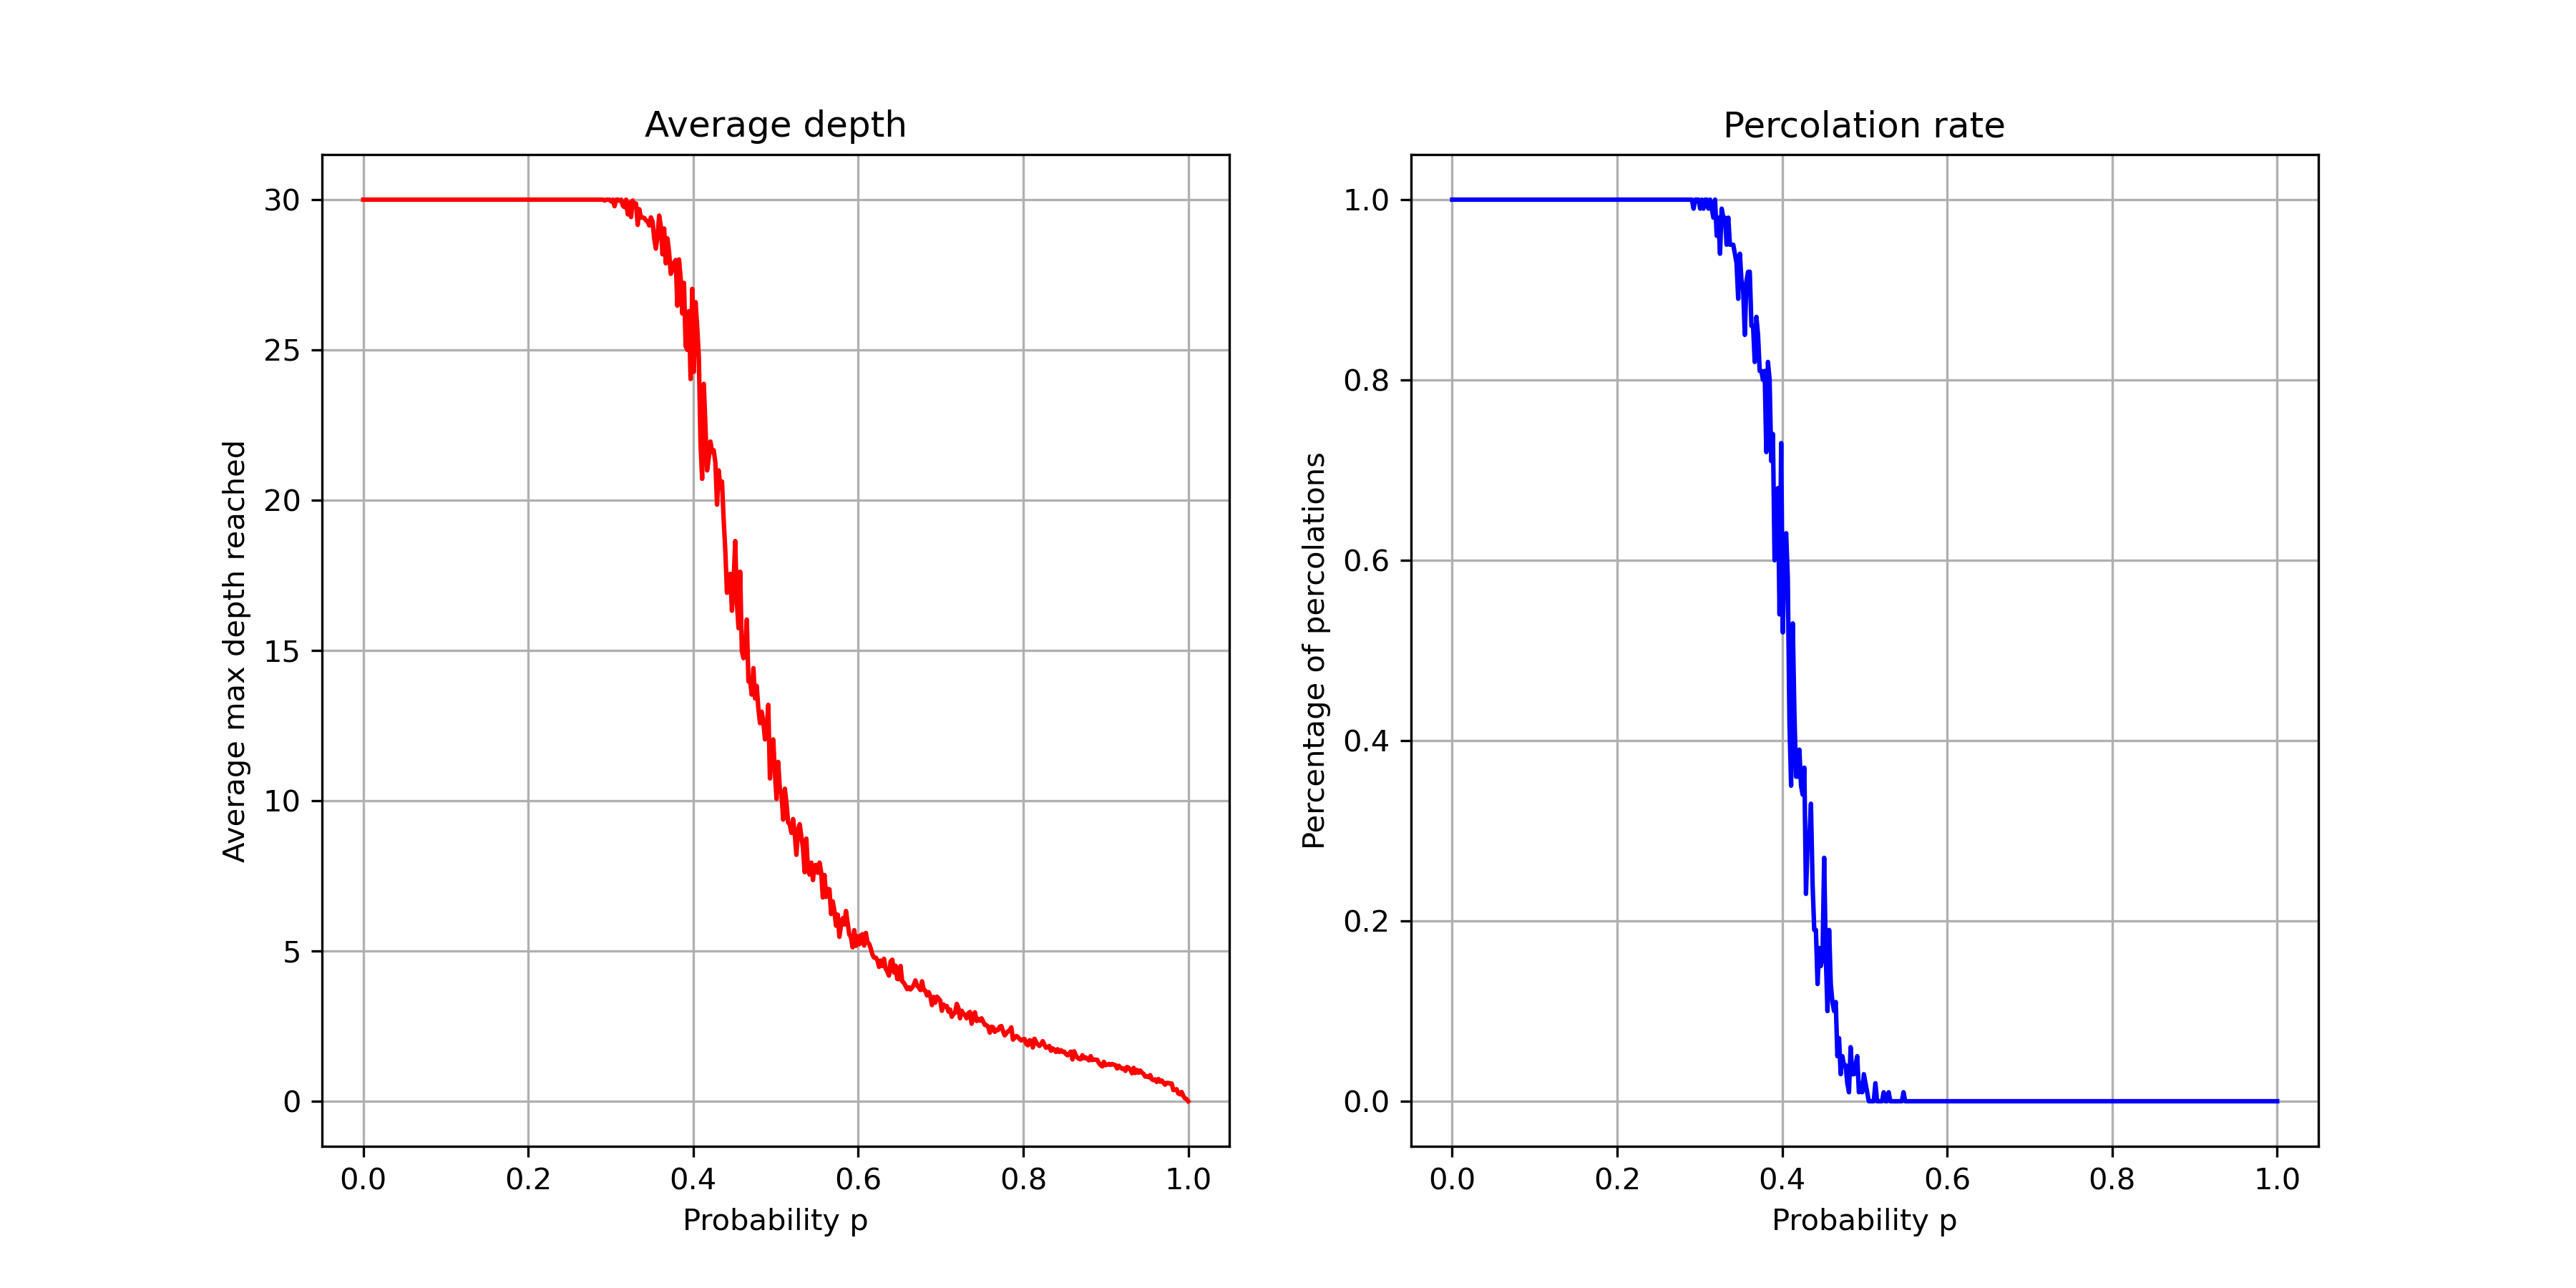
\includegraphics[width=\textwidth]{images/hw_1/depths.png}
    \caption{Ліворуч -- залежність середньої максимальної глибини $d^{\text{avg}}(p)$ від $p$, праворуч -- залежність частки експериментів з перколяцією $\pi(p)$ від $p$.}
    \label{fig:results}
\end{figure}

\end{document}
